\chapter{Introduction and theory}
\label{chap:theory}

\section{The Standard Model of particle physics}
\subsection{Introduction}

The \SM of particle physics was formulated in the second half of the 20$^{\text{th}}$ century. It has been an immensely successful theory, accurately describing all known processes in high energy physics encountered thus far. The \SM is a gauge theory, in particular a \QFT, in which the universe is made up of interacting fields. In this model, the fundamental elements of matter can be represented as relativistic quantum fields, the excitations of which are manifested as particles. Furthermore, the fundamental forces which govern the interactions of matter can be described the exchange of mediator particles. The \SM places the electromagnetic, strong and weak forces into one framework. The only force which is not described not the \SM is gravity, since no viable quantum theory of gravity currently exists. This does not affect the predictive power of the \SM however, since the gravitational force is many orders of magnitude weaker than the other three. The \SM unites the electromagnetic and weak forces into the electroweak force, using the Higgs mechanism to explain the manifest breaking of the underlying symmetry. The Higgs mechanism leads to the prediction of an observable particle, the Higgs boson. All the particles postulated by the \SM have been discovered, capped by the discovery of the Higgs boson in 2012.

%In order to do this, a mechanism ss required to permit the $W^{\pm}$ and $Z$ vector bosons to have mass while allowing the photon to remain masslesss. Such a theory was independently proposed by several theorists~\cite{BroutEnglert,Higgs1,Higgs2,Kibble1,Higgs3,Kibble2}, and is commonly referred to as the Higgs mechanism. In 1964, Higgs postulated that one outcome of this mechanism was that it should yield an observable particle, the Higgs boson~\cite{Higgs2}.

Although the \SM has been very successful as a theory, it falls short of being a “theory of everything", and is clearly incomplete. For instance, it does not accommodate mass terms for neutrinos, which are required to explain the origin of neutrino oscillations observed in many experiments~\cite{SuperK,SNO,DayaBay}. Furthermore, it does not contain a viable candidate for dark matter, which may be needed to explain the mass deficit of the universe~\cite{DM}. Other issues such as the hierarchy problem~\cite{Hierarchy} and the origin of matter-antimatter asymmetry~\cite{Asymmetry} also persist. Clearly, the \SM is incomplete or approximate, and many efforts in modern high energy physics are being made to discover \BSM physics. Many extensions to the  detailed studies of the properties of the Higgs boson could provide valuable insight into the nature or indeed existence of \BSM physics.

%Over the decades, the particles which constitute the SM were discovered: the $\tau$ lepton in 1975~\cite{tauDisc}, the $b$ quark in 1977~\cite{bquarkDisc}, the gluon in 1979~\cite{Gluon1,Gluon2,Gluon3}, the $Z$ and $W^{\pm}$ bosons in 1983~\cite{ZDisc,WDisc}, the $t$ quark in 1995~\cite{tquarkDisc1,tquarkDisc2} and the $\nu_{\tau}$ in 2000~\cite{TauNuDisc}. By the turn of the millennium, all but one particle postulated by the SM had been observed: the Higgs boson, which had proved elusive despite decades of searches. The Higgs search prompted the construction of the Large Hadron Collider (LHC) at CERN, and two multi-purpose detectors, ATLAS and CMS, were designed with the Higgs observation as one of their main physics goals. In 2012, the two experiments jointly announced the observation of a Higgs-like particle of mass $\sim$125 GeV, ending a 50-year interval between postulation and discovery~\cite{CMSHDisc,ATLASHDisc}.


\subsection{Particles and Forces}

 In the \SM, matter is made up a collection of \SpinHalf particles, which are called \emph{fermions}. Fermions come in two types: those wich interact exclusively via the eletroweak force, known as the \emph{leptons} and those which can also interact via the strong nuclear force, known as the \emph{quarks}. The fermions can be arranged into three \emph{generations}, which are identical copies of each other, aside from the masses of the constituent particles. The first generation includes the electron (\Pe), the electron neutrino (\Pnue), the up quark (\Pup) and the down quark (\Pdown). The second generation includes the muon (\Pmu), the muon neutrino (\Pnum), the charm quark (\Pcharm) and the strange quark (\Pstrange). The third and final generation includes the tau (\Ptau), the tau neutrino (\Pnut), the truth or top quark (\Ptop) and the beauty or bottom quark (\Pbottom). Each of the particles mentioned in the list above has a corresponding \emph{antiparticle}, with the same mass and opposite quantum numbers.
The \SM fermions and their properties are displayed in \Tab~\ref{tab:th:fermions}.

\begin{table}[h!]
 \resizebox{\textwidth}{!}{

\begin{tabular}{ |c | c l | c l | c l | }
\hline
type & \multicolumn{2}{|c}{ Generation I} & \multicolumn{2}{|c}{ Generation II} & \multicolumn{2}{|c|}{ Generation III} \\
\hline
  \multirow{4}{*}{leptons} & \multirow{2}{*}{\Large{\Pe}} & $m=0.511\MeV$ & \multirow{2}{*}{\Large{\Pmu}}  &   $m=105\MeV$ &   \multirow{2}{*}{ \Large{\Ptau}}  &   $m=1777\MeV$  \\
                           &                      &   $q=-1$      &   & $q=-1$    &    & $q=-1$   \\ \cline{2-7}
                           & \multirow{2}{*}{\Large{\Pnue}} & $m\sim0\MeV$ & \multirow{2}{*}{\Large{\Pnum}}  &   $m\sim0\MeV$ &   \multirow{2}{*}{ \Large{\Pnut}}  &   $m\sim0\MeV$  \\
                           &                      &   $q=0$      &   & $q=0$    &    & $q=0$   \\
 \hline 
  
  \multirow{4}{*}{quarks} & \multirow{2}{*}{\Large{\Pup}} & $m=2.3\MeV$ & \multirow{2}{*}{\Large{\Pcharm}}  &   $m=1.275\GeV$ &   \multirow{2}{*}{ \Large{\Ptop}}  &   $m=173\GeV$  \\
                           &                      &   $q=+\frac{2}{3}$      &   & $q=+\frac{2}{3}$    &    & $q=+\frac{2}{3}$   \\ \cline{2-7}
                           & \multirow{2}{*}{\Large{\Pdown}} & $m=4.8\MeV$ & \multirow{2}{*}{\Large{\Pstrange}}  &   $m=95\MeV$ &   \multirow{2}{*}{ \Large{\Pbottom}}  &   $m=4.18\GeV$  \\
                           &                      &   $q=-\frac{1}{3}$      &   & $q=-\frac{1}{3}$    &    & $q=-\frac{1}{3}$   \\
 \hline 
  \end{tabular}
}
 \caption{The fundamental \SM particles which constitute all matter in the universe are presented. There are three generations of matter, which are identical copies of each other aside from the mass of the constituent particles. Each generation has two leptons and two quarks. The mass $m$ and electric charge $q$ are indicated for each particle. For every particle in the table, there exists an antiparticle with the same mass but opposite quantum numbers. }
\label{tab:th:fermions}
\end{table}

The fundamental matter particles described above interact via the fundamental forces. There are four known fundamental forces in the universe: the electromagnetic force, the weak nuclear force, the strong nuclear force and the gravitational force. The gravitational force is many orders of magnitude weaker than any of the other forces, and therefore has a negligible effect on the interactions of the \SM particles. Furthermore, no adequate quantum theory of gravity currently exists, therefore it cannot be easily included in the \SM. Therefore, the \SM deals only with the strong, weak and electromagnetic forces.

In the \SM, the fundamental forces, are represented by the exchange of\emph{mediator particles}. In contrast to the \emph{fermions}, the mediators have integer spin. Integer-spin particles are referred to as \emph{bosons}, and in particular the force carriers have spin 1, making them \emph{vector bosons}. 
Each fundamental force is mediated by one or more vector bosons. The electromagnetic force is mediated by the photon (\Pphoton). The weak nuclear force is mediated by the Z-boson (\PZ) and the W-bosons (\PWplus and \PWminus). The strong nuclear force is mediated by the gluons (\Pgluon), of which there are eight, one for each possible colour charge (the strong force equivalent of electric charge).
The forces described by the \SM, along with their mediators, are shown in \Tab~\ref{tab:th:bosons}.

\begin{table}[h!]
 \resizebox{\textwidth}{!}{
\begin{tabular}{ |c | c  | c  | c|  }
\hline
Force &  Indicative Strength & Mediator & Mass  \\
\hline
strong &  $1$ & gluon \Pgluon & 0   \\
\hline
electromagnetic &  $10^{-3}$ & photon \Pphoton & 0   \\
\hline
 \multirow{2}{*}{weak} &  \multirow{2}{*}{$10^{-8}$} & W-boson \PWpm & 80.4 \GeV   \\
                       &                             & Z-boson \PZzero & 91.2 \GeV   \\
\hline
  \end{tabular}
}
 \caption{The three fundamental forces considered by the \SM are presented. For each force, the approximate strength relative to the strong force is shown, assuming two fundamental particles separated by a distance of $10^{-15}\m$. The mediator particle of each force is indicated along with its measured mass.\cite{Thomson:2013zua}}
\label{tab:th:bosons}
  \end{table}

The \Pphoton and \Pgluon are massless, in contrast to the \PWmp and \PZzero, which are massive. This difference is explained via the process of \emph{electroweak symmetry breaking} via the Brout-Englert-Higgs mechanism described in \Sec~\ref{src:th:ewsb}. This mechanism introduces an additional field, which leads to an additional massive observable particle, the Higgs boson. This particle is predicted to be spin-$0$, and therefore it is referred to as a \emph{scalar boson}.

\subsection{Gauge groups of the SM Lagrangian}
\label{sec:th:gauge}

Typically, QFTs are expressed in the Lagrangian formalism. The Lagrangian $\mathcal{L}_{\text{QFT}}$ of a \QFT codifies the dynamics and interactions of its particles. The equations of motion can be extracted using the \ELE. $\mathcal{L}_{\text{QFT}}$ is constructed by considering the nature of the particles involved in the \QFT and imposing the symmetries which the theory ought to display. N\"other's Theorem~\cite{Noether}, one the most important in the study of particle physics, shows a profound relationship between the symmetries of a problem and the laws which govern it: for every symmetry in a Lagrangian, there is an associated conservation law. For example, if we impose that our \QFT should be invariant in time or space, this directly implies that the theory respects conservation of energy or momentum respectively. Similarly, if the \QFT is invariant under rotations in space, angular momentum is conserved. These simple examples illustrate that imposing a symmetry in a Lagrangian will place requirements on how the particles in the theory are allowed to propagate and interact. 

A gauge theory is a particular type of \QFT where local gauge transformations are a symmetry of the Lagrangian. Such gauge symmetries are of principal importance in particle physics, as they lead to the introduction of gauge fields, and thus the gauge bosons which are the mediators of a force. The \SM is in fact a collection of gauge theories. Typically, a gauge transformation takes the form of shifting the quantum mechanical phase of all wavefunctions. It is reasonable to require such transformations to leave the dynamics of the theory intact, since the phase of a wavefunction is never manifest in any physical observable. Thus the Lagrangian of any realistic theory should be \emph{gauge invariant}, i.e. symmetric under phase transformation operations.  

\subsubsection{Quantum Electrodynamics}
A simple example is \QED, where for simplicity we consider a single fermion (others can be trivially added). Fermions are described by the Dirac equation, which, in the Lagrangian formalism, takes the form:

\begin{equation}
\label{eq:th:dirac}
\mathcal{L}_{\textrm{fermion}} = i\overline{\psi} \gamma^{\alpha} \partial_{\alpha} \psi - m\overline{\psi}\psi,
\end{equation}

where $i$ is the imaginary unit, $\psi$ is a Dirac spinor and $\overline{\psi}$ is its adjoint, $m$ is the mass of the fermion, $\gamma^{\alpha}$ represents the Dirac gamma matrices and $\partial_{\alpha}$ is the 4-gradient. 
Requiring \emph{global} gauge invariance means that we require that the Lagrangian is invariant under a global phase transformation

\begin{equation}
\label{eq:th:local_gauge_transform}
\psi \rightarrow \psi'= \psi e^{i\theta},
\end{equation}

where $\theta$ is constant in time and space. This requirement is trivially satisfied by $\mathcal{L}_{\textrm{fermion}}$ :
$$
\mathcal{L}_{\textrm{fermion}} \rightarrow \mathcal{L}_{\textrm{fermion}}'=i\overline{\psi e^{i\theta}} \gamma^{\alpha} \partial_{\alpha} \psi e^{i\theta} - m\overline{\psi e^{i\theta}}\psi e^{i\theta}  =i \overline{\psi } e^{-i\theta} e^{i\theta}\gamma^{\alpha} \partial_{\alpha} \psi - m\overline{\psi} e^{-i\theta} e^{i\theta}\psi  = \mathcal{L}_{\textrm{fermion}},
$$
where it was possible to move $e^{i\theta}$ from the left to the right of the 4-gradient because $\theta$ is a constant. However, there is no particular reason to apply the same transformation throughout space and time. Indeed, the theory should also be invariant under \emph{local} phase transformations $\psi \rightarrow \psi'= \psi e^{i\theta(\vec{x},t)}$, where $\theta(\vec{x},t)$ is now some arbitrary differentiable function.
In this case, one cannot trivially move $e^{i\theta}$ from the left to the right of the 4-gradient. Using the chain rule to differentiate, we can see :
\begin{equation}
\label{eq:th:dirac_lagrangian_not_invariant_local_gauge_transf}
\mathcal{L}_{\textrm{fermion}} \rightarrow \mathcal{L}_{\textrm{fermion}}'=  = \mathcal{L}_{\textrm{fermion}} - \overline{\psi} \gamma^{\alpha} \psi (\partial_{\alpha} \theta(\vec{x},t)),
\end{equation}

So the fermion Lagrangian on its own is not symmetric under local gauge transformations, even though this is a reasonable requirement for any theory which describes our universe. This situation can be remedied by postulating the existence of an additional field $A_\alpha$. We add an additional term to the Lagrangian to account for the interaction of the fermion with this new field, which becomes:
$$
\mathcal{L}_{\textrm{fermion+interaction}} = i\overline{\psi} \gamma^{\alpha} \partial_{\alpha} \psi - m\overline{\psi}\psi  - g_{\textrm{EM}}\overline{\psi}\gamma^{\alpha}\psi A_{\alpha},
$$
where we $g_{\textrm{EM}}$ is a real number which dictates the strength of the electromagnetic interaction.

We impose that $A_\alpha$ changes in a specific way under local gauge transformations. In particular, we ask that:

\begin{equation}
\label{eq:th:photon_gauge}
A_{\alpha} \rightarrow A_{\alpha} + \frac{1}{g_{\textrm{EM}}} \partial_{\alpha} \theta(\vec{x},t),
\end{equation}

According to \Eq~\ref{eq:th:photon_gauge}, the interaction term transforms as:
$$
\mathcal{L}_{\textrm{interaction}} \rightarrow  \mathcal{L}_{\textrm{interaction}}' =  \mathcal{L}_{\textrm{interaction}}  + \overline{\psi} \gamma^{\alpha} \psi (\partial_{\alpha} \theta(\vec{x},t)),
$$
which exactly cancels out the additional term in \Eq~\ref{eq:th:dirac_lagrangian_not_invariant_local_gauge_transf}, thereby restoring invariance under local phase transformations.

One final step is to include a term for the new potential $A_{\alpha}$ propagating through space. Since  $A_{\alpha}$ is a 4-vector, we cannot simply use the Dirac equation. Instead, such fields are correctly described by the Proca equation for spin-1 bosons:

\begin{equation}
\label{eq:th:proca}
\mathcal{L}_{\textrm{boson}} = -\frac{1}{16\pi} F^{\alpha\beta}F_{\alpha\beta} + \frac{1}{8\pi} m_{\textrm{boson}} A^{\alpha} A_{\alpha},
\end{equation}
where $F^{\alpha \beta} =(\partial^{\alpha} A^{\beta} - \partial^{\beta} A^{\alpha})$ and $m_{\textrm{boson}}$ is the mass of the spin-1 boson. 
It is easy to show that $\mathcal{L}_{\textrm{boson}}$ is invariant under local phase transformations so long as we set $m_{\textrm{boson}}=0$, i.e. we require the boson to be massless, and the Proca equation just becomes a simple wave equation.

We now have the full Lagrangian for QED, which is composed of a Lagrangian for a free fermion, a Lagrangian for a free spin-1 boson and a Lagrangian for the interaction between the boson and the fermion. 

\begin{equation}
\label{eq:th:QED_lagrangian}
\mathcal{L}_{\textrm{QED}} = \underbrace{i\overline{\psi} \gamma^{\alpha} \partial_{\alpha} \psi - m\overline{\psi}\psi}_{\textrm{free fermion}}   \overbrace{-\frac{1}{16\pi} F^{\alpha\beta}F_{\alpha\beta}}^{\textrm{free spin-1 boson}}  \underbrace{- g_{\textrm{EM}}\overline{\psi}\gamma^{\alpha}\psi A_{\alpha}}_{\textrm{interaction term}}.
\end{equation}

This was obtained simply by requiring that our theory be invariant under local phase transformations. From this requirement alone came the need for a massless spin-1 boson, which we can now identify as the photon, as well as an interaction between the fermion and the photon, where we can identify the factor multiplying $g_{\textrm{EM}}$, here simply $-1$, as the charge of the fermion. Applying the \ELE to \Eq~\ref{eq:th:QED_lagrangian} yields the usual Maxwell equations for electromagnetism. A convenient way to write this is to define the \emph{covariant derivative} which directly incorporates the interaction term:

\begin{equation}
\label{eq:th:covariant_derivative}
D_{\alpha} = \partial_{\alpha} - i g_{\textrm{EM}}A_{\alpha},
\end{equation}

so that we can re-write \Eq~\ref{QED_lagrangian} more compactly as:

\begin{equation}
\label{eq:th:QED_lagrangian}
\mathcal{L}_{\textrm{QED}} = i\overline{\psi} \gamma^{\alpha} D_{\alpha} \psi - m\overline{\psi}\psi -\frac{1}{16\pi} F^{\alpha\beta}F_{\alpha\beta} -  g_{\textrm{EM}}\overline{\psi}\gamma^{\alpha}\psi A_{\alpha}.
\end{equation}

The local gauge transformation in \Eq~\ref{eq:th:local_gauge_transform} is a multiplication by a real number of modulus 1. This is equivalent to matrix multiplication by a unitary $1\times1$ matrix. The group of all such transformations is the unitary group $U(1)$. It is a general principle that the number of degree of freedom in the underlying symmetry group dictates the number of additional bosons needed to keep the theory locally gauge invariant. This is also the number of types of charge, and here trivially that number is 1.

\subsubsection{Quantum Chromodynamics}

A similar scheme to that used in \Sec~\ref{th:sec:qed} can be used to derive the Lagrangian for \QCD, which codifies the dynamics of the strong force. The situation is more complicated because the underlying group is not $U(1)$ but $SU(3)$. One direct consequence of the more complex group structure is that there are eight degrees of freedom instead of just one. This leads to eight massless gluons in the same way that the single massless photon of \QED was extracted. In \QED, we identified that the interaction between the boson and the fermion was dictated by electric charge; the analogue for \QCD is colour charge, but unlike the electric charge, this cannot simple be represented by a real number, and instead we have eight colours charges, which are linear combinations of \emph{red, antired, green, antigreen, blue, antiblue}. Each \SM quark has three identical copies with different colour charge. Another important difference is that $U(1)$ is abelian while $SU(3)$ is not. The consequence of this is that unlike the \QED photon, which carries no electric charge, the \QCD gluons carry colour charge. Gluons can therefore feel the strong force and self-interact, whereas there is no self-interaction for the photon.

\subsubsection{Electroweak unification}

The Lagrangians for the eletromagnetic and strong forces are both derived by imposing local gauge invariance, leading to the existence of massless bosons which mediate the interaction. There is an analogous theory to \QED and \QCD called \QFD. However, a major achievement of 20$^{\textrm{th}}$ century science was the unification of the electromagnetic and weak forces by Glashow,Weinbeg and Salaam, in what is called \EWT, and also account for some of the odd features of the weak force, such as the fact that it couple to particles differently depending on their \emph{chirality}.

In \EWT, we consider the gauge group $SU(2)_{\textrm{L}} \times U(1)_{\textrm{Y}}$. The $SU(2)$ group has three degrees of freedom, and thus we expect three gauge bosons and three types of charge from imposing local gauge invariance, which we call \emph{weak isospin}, and label $i_1, i_2, i_3$. The subscript in $SU(2)_{\textrm{L}}$ refers to the fact that we only the fact that only left-handed particles may carry weak isospin charge.

The $U(1)$ group has been encountered before in \QED, but in this case the charge considered is not electric charge $q$ but \emph{weak hypercharge} $y$, and we expect a single boson from it. The hypercharge is related to electric charge and weak isospin by the relation $q=y/2 + i_3$. From this realtion it is perhaps already obvious that the conventional weak and electromagnetic forces and their carriers will be 'linear combinations' of the forces and carriers generated by weak isospin and hypercharge. The subscript in $U(1)_{\textrm{Y}}$ refers to the fact that we are considering the hypercharge gauge group.

We can then proceed to deduce the dynamics of this theory by inposing gauge invariance. The case of  $U(1)_{\textrm{Y}}$ is analogous to \QED, and we call the resulting massless spin-1 boson $B_{\alpha}$. It is helpful to think of the fermion spinor as a \emph{singlet}, or a column vector of one spinor. For example, this is labelled $\Pe_{R}$, for the right-handed electron singlet, although the derivation is analogous for other fermions.
For $SU(2)_{\textrm{L}}$, we follow an analogous procedure, but in this case the fermions come in doublets (a column vector of two fermion spinors). Again, using the electron example:
$$
L=\binom{\Pnue}{\Pe}_{L},
$$
which contains the left handed electron and electron neutrino. The fact that no right-handed neutrinos are included in this scheme reflects the fact that no right-handed neutrinos have ever been observed in nature.

By considering gauge invariance of the Lagrangian for the weak isospin double and weak hypercharge singlet, one must introduce gauge bosons with appropiate transformation rules. The resulting gauge fields are $W_{\alpha}^{1},W_{\alpha}^{2},W_{\alpha}^{3}$ and $B_{\alpha}$ respectively. The particles corresponding to these fields have never been observed, because the physical states which we do see (\PWpm, \PZ and \Pphoton) are mixtures of the underlying weak isospin and weak hypercharge gauge bosons:


\begin{equation}
\label{eq:th:electroweak_gauge_bosons}
\PWpm_{\alpha} = \sqrt{\frac{1}{2}}(W_{\alpha}^{1} \mp W_{\alpha}^{2}) ,
\PZzero_{\alpha} = \cos \theta_{W} W_{\alpha}^{3} - \sin \theta_{W} B_{\alpha} ,
A_{\alpha} = \sin \theta_{W} W_{\alpha}^{3} + \cos \theta_{W} B_{\alpha} ,
\end{equation}

where $\theta_{W}$ is the Weinberg angle, which relates strengths of the electromagnetic ($g_{\textrm{EM}}$) and weak ($g_{\textrm{W}}$) forces via the relation $\tan \theta_{W} = g_{\textrm{W}} /g_{\textrm{EM}}$.

\EWT successfully presents the electromagnetic and weak forces as manifestations of the same underlying electroweak force. A similar scheme as the one presented for $e_{R}$ and $L$ above is used to incorporate quarks into this framework. For example, for the first generation of quarks, two right-handed quark singlets $u_{R}$ and $d_{R}$ and one left-handed quark doublet $Q_{L}$ are introduced. An issue arises however, when considering masses of particles. In \QED where the mass of a fermion is given simply by the term $ -m\overline{\psi}\psi$ in the Lagrangian, but the equivalent term, for example for the electron, must account for both the right-handed and left-handed components, which transform differently since one is a singlet and the other is part of a doublet. This breaks the gauge invariance of the fermion mass terms. Furthermore, the gauge bosons which are introduced when applying gauge invariance should be massless to preserve the gauge symmetry. This is the case for the photon, but the \PWpm and \PZzero have experimentally measured masses of the order of 90\GeV. It is clear that some mechanism is needed to account for the masses of these particles. This is provided by \emph{electroweak symmetry breaking} via the Brout-Englert-Higgs mechanism.

\subsection{Electroweak Symmetry Breaking and the Higgs Mechanism}
\label{sec:th:ewsb}

The process which allows the \PWpm and \PZzero to aquire a mass is known as \emph{spontaneous symmetry breaking}. In particular, this occurs in the \SM under the guise of the Brout-Englert-Higgs mechanism. The basis of the symmetry breaking is that one can introduce a complex scalar (spin-0) $SU(2)$ doublet, which we denote as $\phi$, for which the Lagrangian is gauge invariant but the ground state is not. 

Spin-0 boson singlets are described by solutions to the Klein-Gordon equation, which takes the following form in a Lagrangian:
\begin{equation}
\label{eq:th:klein_gordon_lagrangian}
\mathcal{L}_{KG} = \frac{1}{2}(\partial_{\alpha} \Phi)^{*} (\partial^{\alpha} \Phi) - \frac{1}{2} (m_{\Phi})^{2} (\Phi^{*} \Phi)  ,
\end{equation}
where $m_{\Phi}$ is the mass of the sping-0 scalar boson $\Phi$.

We consider a Lagrangian for our doublet $\phi$ of the form:

\begin{equation}
\label{eq:th:higgs_lagrangian}
\mathcal{L}_{\phi} = \frac{1}{2}(D_{\alpha} \phi)^{*} (D^{\alpha} \phi) + \frac{1}{2} \mu^{2} (\phi^{*} \phi) - \frac{1}{4} \lambda^{2} (\phi^{*} \phi) ^{2} ,
\end{equation}

where $\mu$ and $\lambda$ are constants. The covariant derivative $D_{\alpha}$ defined in \Eq~\ref{eq:th:covariant_derivative} has been used here to ensure gauge invariance, except that in this case the interactions with the other gauge bosons, not just the photon but also the $\PWpm, \PZzero$ and glupns, are implicitly taken into account.
The first term of the Lagrangian corresponds to the kinetic part, while the second and third correspond to a potential. Comparing to \Eq~\ref{eq:th:klein_gordon_lagrangian}, the first term of the potential at first appears like a mass term, but it is not: the sign needs to be negative. In the Lagrangian potentials considered so far, the ground state has always been a single point at 0. If we impose $\mu^{2}<0$, the potential has a non-zero \VEV, and the ground state is represented by a circle of minima. In order to re-write the Lagrangian in terms of physical particles, we must expand around one of the minima. Since they are all equivalent, we can pick one which is convenient:

\begin{equation}
\label{eq:th:higgs_vev}
\VEV = \frac{1}{}\sqrt{2} \binom{0}{v} ,
\end{equation}
where $v=\sqrt{- \mu^{2} / \lambda}$. At this stage, any of the minima lying upon the circle of ground states could have been chosen, but in order to find the physical states in the Lagrangian, we have been forced to make a choice. This step breaks the manifest symmetry in the physical states while preserving it in the Lagrangian. 

To obtain the physical states from this Lagrangian, we consider a small perturbation around the \VEV: 

\begin{equation}
\label{eq:th:higgs_vev_perturbation}
\phi = \frac{1}{}\sqrt{2} \binom{0}{v+H} ,
\end{equation}
which can be substituted back into the original Lagrangian in \Eq~\ref{eq:th:higgs_lagrangian}. After some algebra, and expanding out the implicit interactions with the gauge bosons from the covariant derivative, we obtain:

\begin{equation}
\label{eq:th:higgs_lagrangian}
%\mathcal{L}_{\phi} = \frac{1}{2} (\partial_{\alpha} H) (\partial^{\alpha} H) - \frac{1}{2} \mu^{2} H^2 + \frac{v^2}{8}( g_{\textrm{W}} \PWp_{\alpha}\PWp^{\alpha} + g_{\textrm{W}} \PWm_{\alpha}\PWm^{\alpha} + (g^2_{\textrm{W}}+g^2_{\textrm{EM}})  \PZzero_{\alpha}\PZzero^{\alpha}) + ...,
\mathcal{L}_{\phi} = \frac{1}{2} (\partial_{\alpha} H) (\partial^{\alpha} H) - \frac{1}{2} \mu^{2} H^2 + \frac{v^2}{8}( g_{\textrm{W}} \PWp_{\alpha}\PWp^{\alpha} + g_{\textrm{W}} \PWm_{\alpha}\PWm^{\alpha} + (g^2_{\textrm{W}}+g^2_{\textrm{EM}}) \PZzero_{\alpha}\PZzero^{\alpha}) + ...,
\end{equation}
where all terms which resemble mass terms for the gauge bosons have been written and all other terms have been omitted.
Now that the Lagrangian has ben re-written after expansion around a valid minimum, we can identify it with the Klein-Gordon equation in \Eq~\ref{eq:th:klein_gordon_lagrangian}. We can immediately identify the first two terms as the Klein-Gordon equation of a massive scalar boson of mass $\sqrt{2}\mu$: this is the Higgs boson. The other terms are the great success of the Brout-Englert-Higgs mechanism: the \PWpm and \PZzero bosons have aquired masses. The absense of equivalent terms for the photon ang gluons means that they do not aquire masses, which is in accordance with our expectations.

Adding $\mathcal{L}_{\phi}$ to the \SM Lagrangians for \EWT and \QCD maintains local gauge invariance, but allows the weak force mediators to acquire mass. Furthermore, it is possible to add additional gauge invariant terms involving the scalar field. These are known as the Yukawa terms. For example, in the case of the first generation leptons:

\begin{equation}
\label{eq:th:yukawa_coupling}
\mathcal{L}_{\textrm{Yukawa}}= \kappa_{e} (\overline{L} \phi  e_{R} + \overline{e_{R}}) \phi^{\dagger} L \\
                      \quad  =  \kappa_{e} v (\overline{e_{L}} e_{R} + \overline{e_{R}} e_{L} ) +  \kappa_{e}   (\overline{e_{L}} H e_{R} + \overline{e_{R}} H e_{L} ),
\end{equation}
where $\kappa_{e}$ is a real constant. We can immediately recognise the first term as a mass term for the electron and the second as the interaction term between the electron and the Higgs boson. By construction, the strength of the interaction is directly proportinal to the mass of the particle which is considered. Furthermore, the neutrino does not acquire any mass via this mechanism. The scheme described above does not prescribe the masses however: these are free parameters in the theory are must be scpeified from experimental emasurements.

To summarise, using spontaneous symmetry breaking, the Brout-Englert-Higgs mechanism allows one to add gauge-invariant terms to the \SM Lagrangian which permit the $\PWpm$ and $\PZzero$ bosons and the leptons to acquire a mass while leaving the gluons and the photon massless. The outcome is one additional particle, the Higgs boson, which is a massive spin-0 particle, the Higgs boson. The search for the Higgs boson prompted the construction of the \LHC at \CERN, and two multi-purpose detectors, \ATLAS and \CMS, were designed with the Higgs observation as one of their main physics goals. In 2012, the two experiments jointly announced the observation of a Higgs-like particle of mass $\sim$125 GeV, ending a 50-year interval between postulation and discovery~\cite{CMSHDisc,ATLASHDisc}.

 
\section{The Higgs boson}
According to SM, the Higgs boson's coupling with particles is proportional to their masses. As such, its production modes in the environment of the LHC are dominated by interactions involving the heavier particles of the SM. Typically, the Higgs boson is produced by one of the following mechanisms (Fig. \ref{higgs_prod}, whose cross-sections can be seen in Fig. \ref{H_XS_fig}):

  \begin{figure}[h!]

  \centering
  \subfloat[]{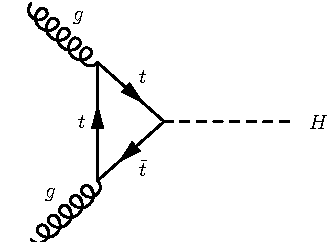
\includegraphics[width=0.3\textwidth]{theoryFigures/ggH.pdf}}
  \subfloat[]{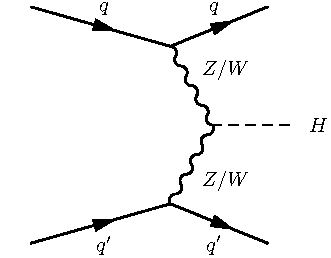
\includegraphics[width=0.3\textwidth]{theoryFigures/vbf.pdf}}\\
  \subfloat[]{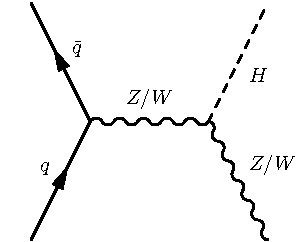
\includegraphics[width=0.3\textwidth]{theoryFigures/wzH.pdf}}
  \subfloat[]{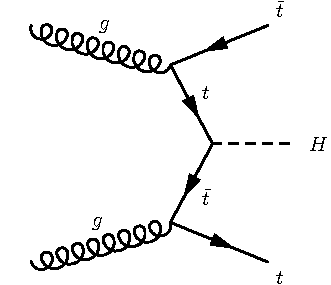
\includegraphics[width=0.3\textwidth]{theoryFigures/ttH.pdf}}
  \caption{Higgs production modes at the LHC: (a) gluon-gluon fusion, via a loop of top quarks, (b) vector boson fusion (VBF), with associated quark production, (c) associated vector boson production and (d) top quark fusion with associated top quark production. }
  \label{fig:theory:higgsproduction}
  \end{figure}

  \newpage
  By the same token, the SM Higgs boson decays to pairs of particles with branching ratios proportional to the square of their mass. The production of a pair of $t$ quarks is not kinematically allowed because their mass is high, so the most likely decay modes are $H \rightarrow ZZ \text{, } W^{\pm}W^{\mp}$, $ b\bar{b}$ and $ \tau^+ \tau^-$. In addition, a small fraction of decays of the Higgs boson ($<1\%$, see Fig. \ref{H_BR_fig}) can occur via a loop diagram to a pair of high-energy photons. The branching fractions and cross sections of these production and decay modes are available in the Handbook of LHC Higgs Cross Sections~\cite{H_XS1,H_XS2}.


 he signal strengths of the various decay modes at the CMS and ATLAS experiments can be seen in Fig. \ref{sig_strength}. Despite fewer than $1\%$ of Higgs boson decays occurring via $H \rightarrow \gamma \gamma$, this channel played a crucial role in the discovery, and remains one of the two most sensitive methods of studying the Higgs boson. This is in part thanks to the excellent performance of the CMS and ATLAS ECALs, which were able to reach similar sensitivities to the $H\rightarrow \gamma \gamma$ decay mode.

  \subsection{History of Higgs boson searches}
  \subsection{Higgs boson at the LHC}
